The results obtained with the embedding + K-NN solution are very promising, as we can see in the t-SNE plot (Figure~\ref{fig:tSNE-plot}, Subsection~\ref{subsec:t-sne-plots}).
\begin{figure}
    \centering
    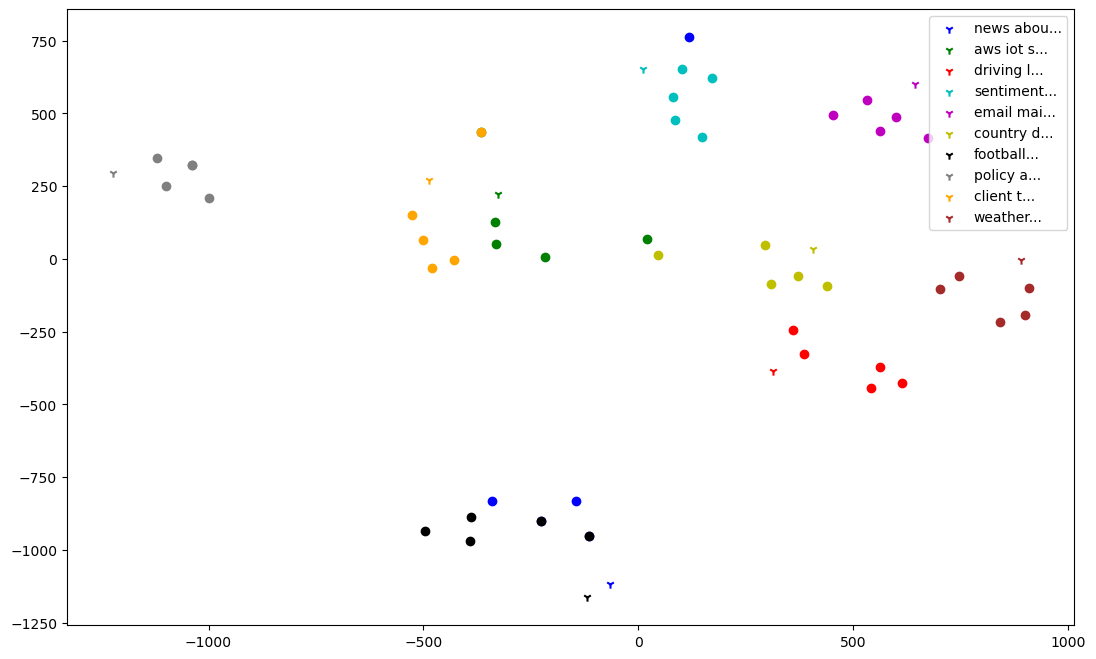
\includegraphics[width=13cm]{/Users/edoriggio/Documents/USI/github/thesis/research/out/plots/SNE}
    \caption{t-SNE Plot}
    \label{fig:tSNE-plot}
\end{figure}
With the \("\)Y\("\) markers representing the queries, and the dots representing the most similar documents found for that query, we can see that the dots and \("\)Y\("\) markers of the same colors are fairly close to each other. \\ \\
Moreover, we performed a validation step with a ground truth.
From the validation step, we concluded that the average precision and recall of the document retrieval (Subsection~\ref{subsec:evaluation}) are:
\[\overline{P} = 0.6 ~~~~~~ R = 1.0\]
This validation was done on 10 different queries.
The position in which each ground truth appeared in the searches can be found in Figure~\ref{fig:ground-truth-eval}.
\begin{figure}
    \begin{verbatim}
  Position in which the ground truth was found:

      "NFL v3 Ply-by-Play" was found at position #1
      "AWS IoT Secure Tunneling" was found at position #4
      "Transport Department" was found at position #4
      "Text Analytics & Sentiment Analysis API | api.text2data.com" was
        found at position #4
      "MailboxValidator Free Email Checker" was found at position #1
      "Interzoid Country Data Standardization API" was found at position #1
      "Soccer v3 Projections" was found at position #1
      "PolicyClient" was found at position #1
      "NetworkManagementClient" was found at position #3
      "Interzoid Get Weather City API" was found at position #2
    \end{verbatim}
    \caption{Ground Truth Evaluation}
    \label{fig:ground-truth-eval}
\end{figure}
As we can see, all ground truths we found in the top 5 results -- hence $R = 1.0$.
The validation on the ground truth, though, does not paint the full picture of the capabilities this solution offers.
For example, Figure~\ref{fig:query-example} represents the top 5 documents returned by the information retrieval system if we try searching using the query: \("\)american sports news\("\).
\begin{figure}
    \begin{verbatim}
  These are the top 5 results of the query "american sports news":

      1. NFL v3 Play-by-Play     v.1.0   [67%]
      2. News Plugin             v.1     [66%]
      3. Soccer v3 Projections   v.1.0   [64%]
      4. MLB v3 Projections      v.1.0   [64%]
      5. NFL v3 Scores           v.1.0   [64%]
    \end{verbatim}
    \caption{Example Output of a Query}
    \label{fig:query-example}
\end{figure}
As we can see in the results above, the engine is able to recognize that both the \textit{NFL} and the \textit{MLB} are professional American sport leagues.
The former being the National Football League, and the latter being the Major League Baseball.
Moreover, it is also able to understand that soccer is a sport and return it. \\ \\
As can be seen both in the average precision ($\overline{P} = 0.6$), and the above example, there are still some noisy results that match part or none of the queries, but this is acceptable.
The reason is that this is not the only means of searching.
To further filter the documents returned by the information retrieval system, we will implement a DSL for the user to specify filters to apply to the NL query.
